\documentclass[UTF8]{article}
\usepackage{CTEX}
\usepackage[T1]{fontenc}
\usepackage{textcomp}

\usepackage{amsmath}
\usepackage{amsfonts}
\usepackage{mathrsfs}
\usepackage{pythonhighlight}
\usepackage{hyperref}
\usepackage{graphicx}
\usepackage{float}

\title{Python语言程序设计期末报告}
\author{-}
\date\today

\begin{document}
\maketitle
\tableofcontents

\section{程序功能简介}

本程序采用python编程语言和tkinter库进行图形界面开发,属于小游戏。在本游戏中,玩家操纵红色的光标躲避由上而下翻滚的方块,防止被翻掉,并可释放一些技能来消除一些方块。目前,功能已经较为完善。该游戏起名为keep away from the stars属历史原因。

\subsection{游戏界面}
\begin{center}
\begin{figure}[H]
\centering
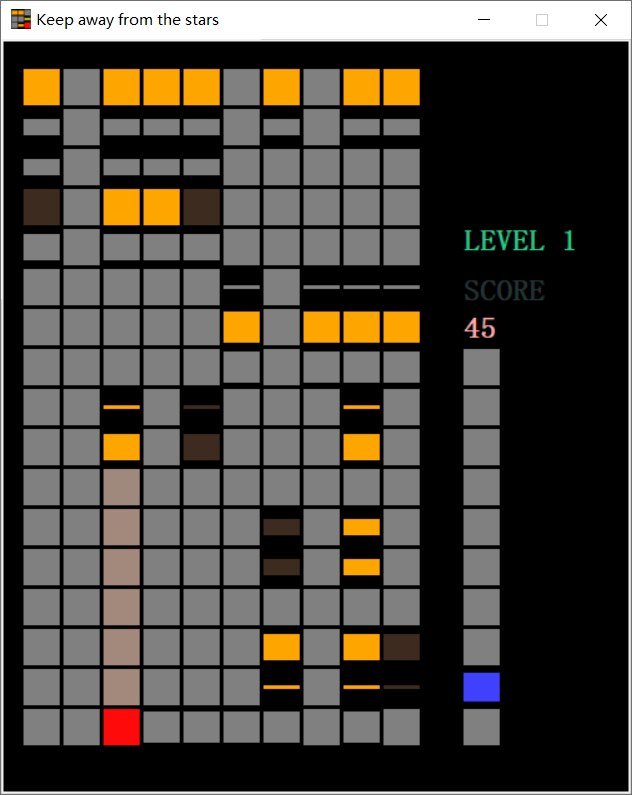
\includegraphics[scale=0.52]{fig_1.png}
\end{figure}
\end{center}
游戏界面如上图所示。其中,左侧的$10\times 17$方块是游戏操作区,玩家可以操纵光标在最下方的一行移动。右侧的$1\times 10$方块是能量条,显示了目前能量的储备。当能量储备充足时,玩家可以使用相关技能。另外,右上角的文字显示了目前所在的等级、得分等信息。

\subsection{游戏的控制}

玩家可以通过键盘的\textleftarrow、\textrightarrow箭头操纵光标移动。当右侧有超过两格能量时,可以通过\textdownarrow箭头使用技能挡住上方最近的一个橙色方块和其后附近的橙色方块。当能量只有一格时,此技能弱化为消除上方最近的一个方块。类似地,在有超过三格能量时可以用\textuparrow箭头反转此列所有的橙色方块。但以上的技能对深褐色的方块无效。有超过四格能量时,可以按空格键消除全屏的橙色方块。

在游戏进展到一定阶段时,会自动切换至下一关卡。

\begin{figure}[htbp]
\centering
\begin{minipage}[t]{0.48\textwidth}
\centering
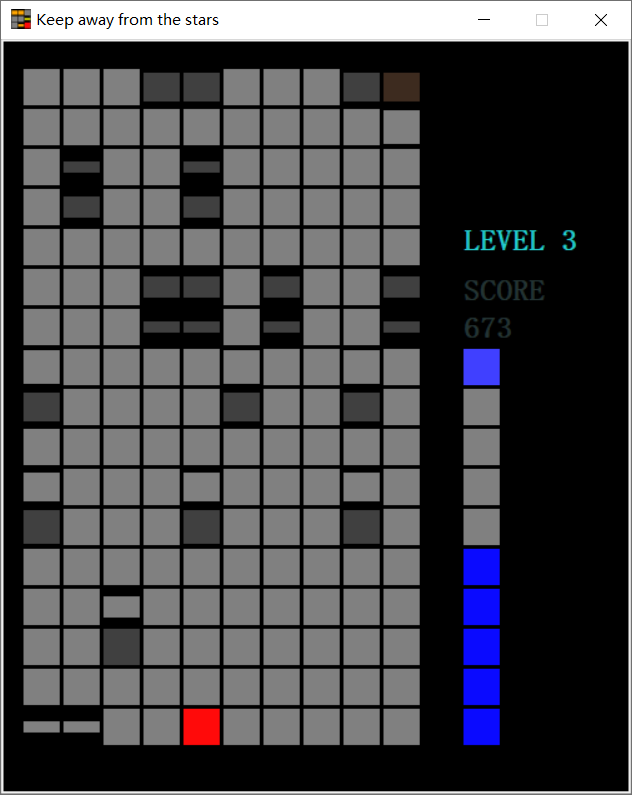
\includegraphics[scale=0.3]{fig_2.png}
\caption{使用空格键的技能}
\end{minipage}
\begin{minipage}[t]{0.48\textwidth}
\centering
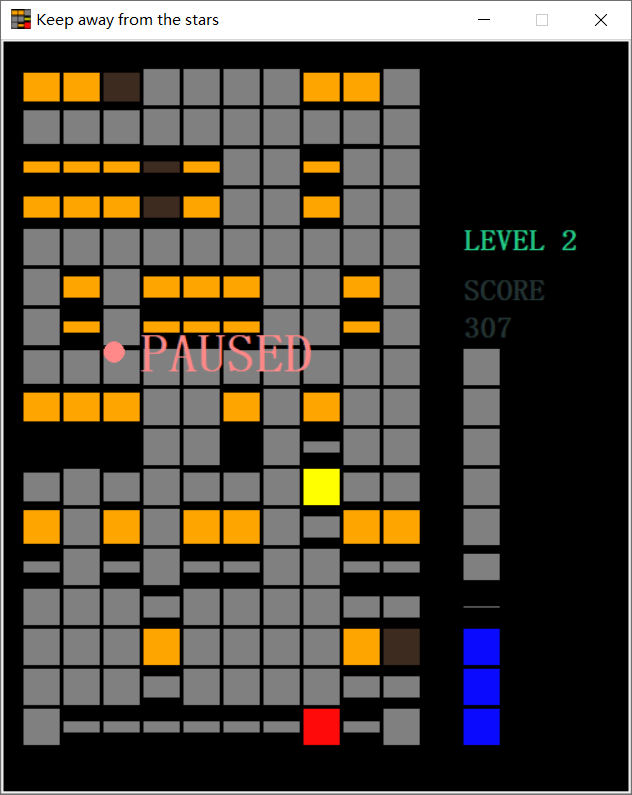
\includegraphics[scale=0.3]{fig_3.png}
\caption{暂停页面}
\end{minipage}
\end{figure}

\begin{figure}[htbp]
\centering
\begin{minipage}[t]{0.48\textwidth}
\centering
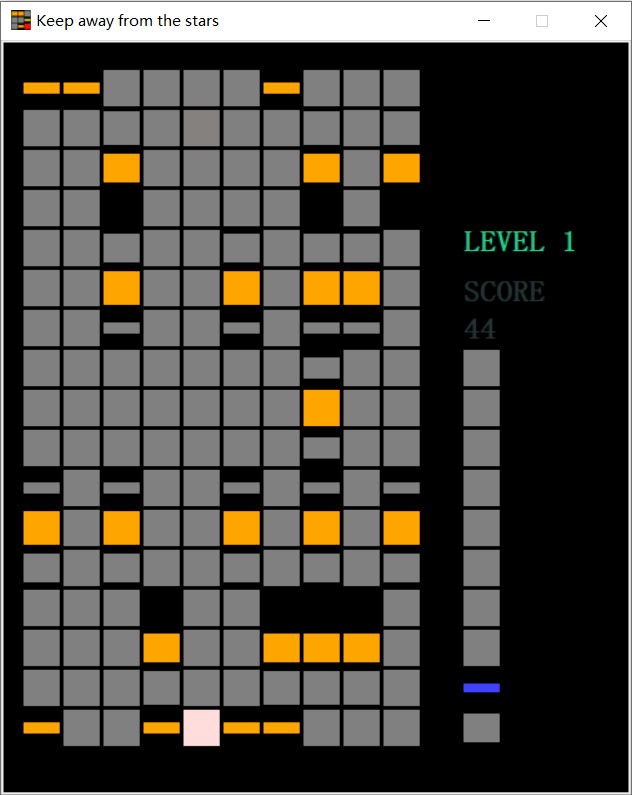
\includegraphics[scale=0.3]{fig_4.png}
\caption{无法移动时,光标会闪烁提示}
\end{minipage}
\begin{minipage}[t]{0.48\textwidth}
\centering
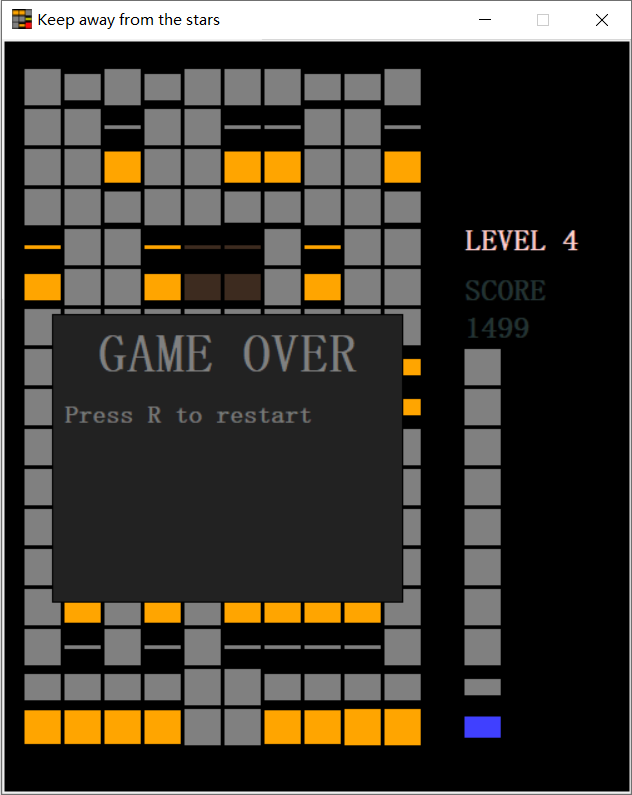
\includegraphics[scale=0.3]{fig_5.png}
\caption{游戏结束页面}
\end{minipage}
\end{figure}

玩家可以按下键盘\texttt{P}键来暂停或继续游戏。当游戏结束后,可按\texttt{R}键重新开始游戏。

\section{程序设计思路}
本程序分为两个模块,其中$\texttt{game.py}$处理游戏运作的逻辑,$\texttt{window.py}$处理游戏界面的绘制,前者可以独立于后者运行。

\subsection{逻辑处理}

程序的运作方式为,首先初始化一个表格用来记录所有方块的信息,然后再通过\texttt{update()}方法更新下一时刻的信息。具体实现为,依次调用每个小方块的\texttt{tic}方法,根据其自身和周围方块的属性按需求更新其状态。有关的属性包括颜色\texttt{color}、\texttt{tmp}、\texttt{tmp2}等等。此外,\texttt{appearance}属性规定了此方块的样式。

游戏整体的状态的记录在\texttt{game}类中,而小方块的状态则记录在\texttt{block}类中。

\subsubsection{小工具} 为了方便,引入
\begin{python}
const = lambda x: lambda *y, **k: x
\end{python}
该函数是组合子$K := \lambda a.\lambda b. a$,\texttt{const(a)}。其作用是生成一个函数,忽略所有的参变量,而返回\texttt{a}本身。

设定了两个异常
\begin{python}
class FailedException(BaseException):
    pass

class InsufficientEnergyException(BaseException):
    def __init__(self, e):
        self.e = e
\end{python}
留作备用。

\subsubsection{方块} 初始化时,预设\texttt{tmp}和\texttt{tmp2}属性为\texttt{0},并将颜色设定为白色。
\begin{python}
    def __init__(self):
        self.color = block.WHITE
        self.tmp   = 0
        self.tmp2  = 0
\end{python}

其中,对颜色进行设定时,会同时指定该方块在更新的方式和输出的方式。具体实现由\texttt{property}装饰器实现:
\begin{python}
    @property
    def color(self):
        return self._color
    
    @color.setter
    def color(self, value):
        self._color = value
        self.tic_function = tic_functions[value]
        self.rep_function = apr_functions[value]
\end{python}
而形如\texttt{block.WHITE}本身则是定义在$block$类中的类属性。如
\begin{verbatim}
    WHITE = 0
    RED = 1
    ...
    BRASS = 13
\end{verbatim}
等等。

\verb|tic_functions|和\verb|apr_functions|是预设好的函数表。在方块需要更新时,就会直接调用这些函数:
\begin{python}
    def tic(self, t):
        self.tic_function(self, time=t)
        
    @property
    def appearance(self):
        return self.rep_function(self)
\end{python}
这样处理是为了方便将本身作为参数传进函数表中的函数,以便于后续的操作。

\subsection{游戏的初始化}

游戏本体储存在\verb|base_game|类和一些衍生的类中。\verb|base_game|的初始化过程如下:
\begin{python}
    def __init__(self):
        self.blocks = [[block() for x in range(1, WIDTH+1)] for y in range(HEIGHT+1)]
        self.family = lambda x, y: self.blocks[y][x-1]
        for y in range(HEIGHT+1):
            for x in range(1, WIDTH+1):
                b = self.family(x, y)
                b.is_far_left  = x == 1
                b.is_far_right = x == WIDTH
                b.is_bottom    = y == 0
                b.is_top       = y == HEIGHT
                
                b.left  = b.is_far_left  or self.family(x-1, y)
                b.right = b.is_far_right or self.family(x+1, y)
                b.up    = b.is_top       or self.family(x, y+1)
                b.down  = b.is_bottom    or self.family(x, y-1)
        self.cursor = self.family(4, 0)
        self.cursor.color = block.RED
        self.cursor.tmp = MAX_TMP // 2

        [...]
        self.time= 0
\end{python}
它定义了一个二维数组\texttt{self.blocks},存储当前的所有方块的信息。而\texttt{self.family}则是一个为方便访问这些信息而设定的函数。在这些方块的信息设定完了以后,需要指定其是否为边缘的方块,以及对临接的方块的引用等,这些信息在上述双层\texttt{for}循环中设定。随后的三行设定玩家操纵的方块位于最下一行左数第四个,设定其颜色和\texttt{tmp}值。类似地,建立一个数组记录能量条的信息(稍后会讲),然后指定此时的时间为\texttt{0}。

\subsubsection{更新方块}
这些函数存储在函数表中,它们接受一个参数\texttt{self}指定方块本身的对象,以及任意个关键字参数\verb|**kw|。将一些额外的信息归于关键字参数处理的原因在于,有一些方块需要额外的信息才能更新,而另一些却没有必要用。这样写在需要引入新的参数时,可以少改动一些原有的代码。

完整的函数表如下:
\begin{python}
tic_functions = [tic_white, tic_red, tic_orange, tic_blue, tic_blue_static, tic_blue_falling, tic_shining, tic_blue_transiting, tic_green, tic_green_fading, tic_yellow, tic_bistre, tic_grey, tic_brass]
\end{python}

有一些方块在更新的过程中什么也不用做,故将它们设置为空函数即可。
\begin{python}
tic_white = tic_blue_static = const(None)
\end{python}

而另一些方块在更新时,需要访问自身乃至周边的方块的属性。以如下的方块为例:

\paragraph{橙色}在更新时,需要指定其翻转的进度(调整\texttt{tmp}值)。当翻转到一定时刻(\texttt{tmp}值达到预设的\verb|TMP_1|)时,需要考虑调整下面的方块的信息。若下面还有方块,且该方块为白色,那么就将其设定为未开始翻转的橙色方块的样式;若下面的方块为红色,那么便修改它的属性使其成为无法移动的格式。翻转结束(\texttt{tmp}值达到\texttt{0})之后,便将自己的颜色调整回白色。

注意到,若橙色的方块在调整下面的方块时发现其颜色不是红色或白色,那么它就不会进行向下蔓延的处理,从而被“挡住”。

相关代码如下:
\begin{python}
def tic_orange(self, **kw):
    self.tmp = self.tmp - 1
    if self.tmp == TMP_1:
        if not self.is_bottom:
            if self.down.color == block.RED:
                self.down.tmp2 = block.ORANGE
            elif self.down.color == block.WHITE:
                self.down.color = block.ORANGE
                self.down.tmp   = MAX_TMP
    elif self.tmp == 0:
        self.color = block.WHITE
\end{python}

\paragraph{红色} 在更新时,若处于正常状态(\texttt{tmp2}的值和\texttt{block.WHITE}相等),则什么也不用做;但若异常状态,则开始该方块的翻转。当方块被彻底反转过去时,抛出\texttt{FailedException}异常,从而触发游戏的终止机制。

\begin{python}
def tic_red(self, **kw):
    if self.tmp2 != block.WHITE:
        self.tmp = self.tmp - 1
        if self.tmp == 0:
            raise FailedException
\end{python}

\paragraph{绿色} 首先更新其翻转的进度(调整\texttt{tmp}值)。当翻转到一定时刻(\texttt{tmp}值达到预设的\verb|TMP_1|)时,需要考虑调整上面的方块的信息。若上面还有方块,且该方块为白色,那么就将其设定为未开始翻转的绿色方块的样式;若上面的方块不是白色,那么就将自己的颜色调整为正在褪色的绿。翻转结束(\texttt{tmp}值达到\texttt{0})之后,便将自己的颜色调整回白色。

\begin{python}
def tic_green(self, **kw):
    self.tmp = self.tmp - 1
    if self.tmp == TMP_1:
        if not self.is_top:
            if self.up.color == block.WHITE:
                self.up.color = block.GREEN
                self.up.tmp   = MAX_TMP
            else:
                self.color = block.GREEN_FADING
                self.tmp = MAX_TMP
    elif self.tmp == 0:
        self.color = block.WHITE
\end{python}

\paragraph{正在褪色的绿} 首先,在合适的时刻(时间参数,即\verb|kw['time']|被\texttt{3}整除时)更新其褪色的进度(调整\texttt{tmp}值)。彻底褪色(\texttt{tmp}值达到\texttt{0})之后,便将自己的颜色调整回白色。

\begin{python}
def tic_green_fading(self, **kw):
    if kw['time'] % 3 == 0:
        self.tmp = self.tmp - 1
    if self.tmp == 0:
        self.color = block.WHITE
\end{python}

\paragraph{深褐色} 深褐色的方块更新方式与橙色极为相似,区别在于需要调整下方方块时,无论是什么方块都会进行调整,且调整方式为将下方方块的颜色转变为深褐色(若它不是红色)。这就塑造出了一种普通技能放出的方块无法对深褐色方块进行抵挡的效果。

\begin{python}
def tic_bistre(self, **kw):
    self.tmp = self.tmp - 1
    if self.tmp == TMP_1:
        if not self.is_bottom:
            if self.down.color == block.RED:
                self.down.tmp2 = block.BISTRE
            elif True:
                self.down.color = block.BISTRE
                self.down.tmp   = MAX_TMP
    elif self.tmp == 0:
        self.color = block.WHITE
\end{python}

还有一些其它的方块更新函数,其具体定义详见源码,它们设定的方式也是类似的。

对于基础版的游戏,更新时,应重设此时的时间,并分别对每一个方块进行更新。
\begin{python}
        self.time = self.time + 1
        for s in self.blocks:
            for t in s:
                t.tic(self.time)
\end{python}
对于能量条的部分,也应在同时进行更新。
\begin{python}
        for u in self.energy_bar:
            u.tic(self.time)
\end{python}

在一定时刻,也会更新最顶端的方块,使其出现一定量的橙色和深褐色方块。另外,也应执行回调的函数以增加分数
\begin{python}
        if self.time % (MAX_TMP//4) == 0:
            scorecallback(1)
        if self.time % MAX_TMP == 0:
            for x in range(1, WIDTH+1):
                b = self.family(x, HEIGHT)
                if b.color == block.WHITE:
                    if random() < 2/7:
                        b.color = block.ORANGE
                        b.tmp = MAX_TMP
                    elif random() < 1/20:
                        b.color = block.BISTRE
                        b.tmp = MAX_TMP
\end{python}

\subsection{玩家对游戏的操作}

\paragraph{移动光标} 处理光标移动时,需要判断玩家试图让光标移动的方向是否有空间,若有,则执行移动游戏中存储的光标位置的引用,调整相关方块的颜色和\texttt{tmp}值等操作。若不可向此处移动,则调用\texttt{failcallback}函数,给玩家做出反馈。例如,向左移动的代码如下:
\begin{python}
    def move_cursor_left(self, failcallback=lambda:print('Cannot move left')):
        if not self.cursor.is_far_left \
            and self.cursor.left.color == self.cursor.tmp2 == block.WHITE:
            self.cursor.color = block.WHITE
            self.cursor.tmp = 0
            self.cursor = self.cursor.left
            self.cursor.color = block.RED
            self.cursor.tmp = MAX_TMP // 2
            self.cursor.tmp2 = block.WHITE
        else:
            failcallback()
\end{python}

向右移动的操作是类似的。

\paragraph{使用技能} 首先,将使用能量的功能封装到了一个方法中:
\begin{python}
        try:
            e = [b.color for b in self.energy_bar].index(block.BLUE)
        except ValueError:
            raise InsufficientEnergyException(-1)
        if e >= n:
            self.energy_bar[e-n].color = block.SHINING
            self.energy_bar[e-n].tmp = 5
            self.energy_bar[e-n].tmp2 = block.BLUE
            for b in self.energy_bar[e-n+1:e]:
                b.color = block.SHINING
                b.tmp = 5
                b.tmp2 = block.WHITE
            self.energy_bar[e].color = block.BLUE_TRANSITING
            self.energy_bar[e].tmp2 = 5
        else:
            raise InsufficientEnergyException(e)
\end{python}
它检测当前蓝色方块的位置,若没有蓝色方块,\texttt{index}会引发\texttt{ValueError},那么说明此时不得释放技能,抛出异常\texttt{InsufficientEnergyException(-1)}。接下来,根据蓝色方块的位置判断此刻有多少能量可用,若能量不足,则抛出异常\texttt{InsufficientEnergyException(e)},其中\texttt{e}是检查出的此刻的能量数。否则会执行代码,将消耗掉的能量方块标记为闪烁的方块,并规定闪烁的次数(通过调整\texttt{tmp}值)。现存的蓝色方块将被改变为正在掉落的蓝色方块。通过改变\texttt{tmp2}值,可以实现在最下方闪烁的方块在闪烁后,将其变回蓝色。

以使用mono技能为例。首先尝试使用两点能量,若能量充足,则正常使用技能,即在光标上放置一个绿色方块。与此同时,调用回调函数加25分。
\begin{python}
    def powerup_mono(self, scorecallback=partial(print, "Increase score by"), failcallback=lambda:"energy is insufficient"):
        try:
            self.use_energy(2)
            self.cursor.up.color = block.GREEN
            self.cursor.up.tmp = MAX_TMP
            scorecallback(25)
\end{python}
若能量不足,则尝试使用一点能量,使用较弱的技能,即在光标上方防止一个青铜色的方块。与此同时,调用回调函数加15分。
\begin{python}
        except InsufficientEnergyException:
            try:
                self.use_energy(1)
                self.cursor.up.color = block.BRASS
                self.cursor.up.tmp = MAX_TMP // 2
                scorecallback(15)
\end{python}
若能量仍然不足,那么调用表示放技能失败的回调函数,给玩家一个反馈。
\begin{python}
            except InsufficientEnergyException:
                failcallback()
\end{python}

另外两种技能的定义详见源码。

\subsection{方块的样式}

方块的样式有函数表\verb|apr_functions|中的函数所确定。这些函数接收一个变量\texttt{self},即方块对象本身,返回一个元组\texttt{(color, fpos)},其中\texttt{color}是一个表示rgb颜色的三元组,而\texttt{fpos}则是一个函数,接收本方块的相对位置\texttt{(x,y)},并返回方块四个角所在的位置\texttt{(x1,x2,y1,y2)}。方块的样式可以抽象出三种类型:正翻转的方块、静止的方块和正改变颜色的方块。其中静止的方块只需要颜色信息,故定义为
\begin{python}
static_block = lambda color: (color, lambda x, y:(x-BLOCK_SIZE_H, y-BLOCK_SIZE_H, x+BLOCK_SIZE_H, y+BLOCK_SIZE_H))
\end{python}
翻转的方块依靠\texttt{tmp}值用正弦函数计算翻转的角度,以及是正面还是背面朝上。考虑到此方法被调用次数较多,但实际上参数的种类有限,故采用了\texttt{functools}包中的\verb|lru_cache|生成装饰器来记忆。定义如下:
\begin{python}
@lru_cache()
def vertically_flipped_block(color, front, tmp):
    h0 = BLOCK_SIZE_H*cos(tmp/MAX_TMP*2*pi)
    if h0 >= 0:
        c = front
        h = h0
    else:
        c = color
        h = -h0
    return c, lambda x, y: (x - BLOCK_SIZE_H, y - h, x + BLOCK_SIZE_H, y + h)
\end{python}
正改变颜色的方块则根据\texttt{tmp}及开始和结束时的rgb颜色线性插值算出此刻的颜色值,定义如下
\begin{python}
@lru_cache()
def transiting_block(color_0, color_max, tmp):
    r0, g0, b0 = color_0
    rm, gm, bm = color_max
    m = tmp/MAX_TMP
    l = 1.0 - m
    return static_block((round(l*r0+m*rm), round(l*g0+m*gm), round(l*b0+m*bm)))
\end{python}

有了这些工具,就可以方便地定义一系列的方块的展示函数。例如
\begin{python}
@lru_cache()
apr_white = const(static_block((128,128,128)))

apr_orange = lambda self: vertically_flipped_block((255,165,0),(128,128,128), self.tmp)
\end{python}
确定了白色方块展示为灰白色的静止方块,橙色方块展示为正翻转的方块,其正面时橙色,背面是灰白色,翻转的系数由\texttt{self.tmp}确定。

剩下的展示函数详见源码。

\subsection{测试模块}

\texttt{game}类提供了\verb|__repr__|函数用来在REPL界面中展现对象目前的状况,在命令行中打印一张表格来显示各个方块的颜色、\texttt{tmp}值等信息。

\subsection{更多的关卡}

导出的关卡通过继承\verb|base_game|实现。在\verb|derived_game|中,需要调用原来的游戏才能初始化,不得直接初始化。这个过程会复制原关卡的方块表、光标位置等信息。\verb|lv2_game|、\verb|lv3_game|和\verb|lv4_game|继承了\verb|derived_game|。并重载\texttt{update}方法,从而实现了增添橙色和深褐色方块的数量、加速等功能,提升游戏的挑战性。

\subsection{界面的绘制}

游戏界面存储在\texttt{window.py}中。这一部分主要包括\texttt{window}类,构建\texttt{window}类时就会通过\texttt{tkinter}包中的组件来展现出游戏的窗口界面。由于本部分涉及\texttt{tkinter}组件调用的部分较多,因篇幅有限,故只讲程序的答题思路。

\begin{python}
@lru_cache()
def color_num(rgb):
    return '#%02x%02x%02x' % rgb
\end{python}
以上\verb|color_num|辅助函数将rgb转化为与\texttt{tkinter}兼容的颜色字符串格式。

\paragraph{初始化}
\begin{python}
class window:
    [...]
    def __init__(self):
        self.root = tk.Tk()#tk.Toplevel()
        self.root.title('Keep away from the stars')
        self.root.iconbitmap('res/icon.ico')
        self.root.resizable(0, 0)
        [...]
        self.start_game()
        self.root.mainloop()
\end{python}
在\texttt{window}类的构建函数中,确定了窗口的大小、画布的位置等信息,然后调用\verb|start_game|方法启动游戏。随机进入事件监听循环。

\paragraph{启动}
\begin{python}
    def start_game(self):
        self.game = game.base_game()
        self.game_status = window.PLAYING
        self.canvas.itemconfig(self.level_id, text="LEVEL 1", fill='#23cc88')
        self.time = 0
        self.score = 0
        self.score_blink_tmp = 0
        self._stressing_tmp = 0
        def add_score(n):
            self.score = self.score + n
            if n >= 10:
                self.score_blink_tmp += 16
        self.add_score = add_score
        self.paused = False
        self.drawing = False
        self.draw()
\end{python}
在\verb|start_game|方法中,需要设置游戏状态、关卡、分数和一些辅助变量的初始值,设定增加分数的回调函数,并调用\texttt{draw}方法开始绘制的循环。

\paragraph{主循环}
\begin{python}
    def draw(self):
        self.canvas.after(window.REFRESH, self.update_method)
        if self.drawing:
            #print('jammed at T+%d' % self.game.time)
            return
        self.drawing = True
        
        [...] # code about upgrading
        
        try:
            self.game.update(scorecallback=self.add_score)
        except game.FailedException:
            self.game_status = window.GAME_OVER
            
        self.canvas.itemconfig(self.score_id, text="%d" % self.score, fill=['#233333', '#ffaaaa'][(self.score_blink_tmp//4) % 2])
        if self.score_blink_tmp > 0:
            self.score_blink_tmp = self.score_blink_tmp - 1
        
        i = 0
        for y in range(game.HEIGHT+1):
            for x in range(1, game.WIDTH+1):
                b = self.game.family(x, y)
                color, fpos = b.appearance
                self.canvas.coords(self.rects_id[i], fpos(x*32, window.IM_Y-y*32))
                if b == self.game.cursor and self.stressing:
                    self.canvas.itemconfig(self.rects_id[i], fill='#ffdddd')
                else:
                    self.canvas.itemconfig(self.rects_id[i], fill=color_num(color))
                i = i + 1

        [...] # code about drawing the energy bar
        
        self.drawing = False
\end{python}
在\texttt{draw}方法中,首先确定在间隔一段时间后,接下来会调用的函数。然后检查并设置辅助变量\texttt{self.drawing}(该辅助变量的作用类似于互斥锁),防止该函数会在同时被多次调用从而引发错误。接下来,调用\texttt{game}模块的接口更新游戏信息,若传出错误,游戏失败,则设置游戏的状态\verb|self.game_status|,该属性的改变会影响到接下来用来更新的函数\verb|self.update_method|的改变。然后依次处理是否应升级、显示分数、显示方块等,最后将调整辅助变量\texttt{self.drawing},以保证下一次绘制能够正常运作。

\paragraph{键盘信息的读取} 这一部由\verb|on_key|方法处理。大致结构如下
\begin{python}
    def on_key(self, event):
        if self.game_status == window.PLAYING:
            if event.keycode == 32:
                self.game.powerup_ninja(scorecallback=self.add_score, failcallback=self.stress)
            elif event.keycode == 37:
                self.game.move_cursor_left(failcallback=self.stress)
            [...]
            elif event.keycode == 80:
                self.game_status = window.PAUSED
        [...]
        elif self.game_status == window.GAME_OVER:
            if event.keycode == 82:
                self.continue_instruction()
\end{python}
当玩家按下按键时,此方法就会被\texttt{tkinter}调用。调用时,会根据此时游戏的状态进入相应的分支,然后处理相应的按键信息。

\texttt{window}类还有一些诸如控制暂停页面和游戏结束页面的代码,限于篇幅有限不再一一赘述。

\begin{python}
@lru_cache()
def color_num(rgb):
    return '#%02x%02x%02x' % rgb
\end{python}

\section{结果分析}

游戏可以通过python解释器运行,也可以通过打包好的可执行文件运行。各个功能正常稳定。本人试玩时,达到过约1500分。

\newpage

\section{程序完整源码}
此程序与本人的Github页面\href{https://github.com/sclereid/keep-away-from-the-stars}{https://github.com/sclereid/keep-away-from-the-stars}同步。另外,在\href{https://github.com/sclereid/keep-away-from-the-stars/releases}{https://github.com/sclereid/keep-away-from-the-stars/releases}有打包好的程序可供直接下载运行。
\subsection{\texttt{game.py}的内容(共$448$行)}

\begin{python}
# -*- coding: utf-8 -*-

from random import random
from math import cos, pi
from functools import lru_cache, partial

WIDTH = 10
HEIGHT = 16
MAX_TMP = 40
TMP_1 = 26
BLOCK_SIZE_H = 15
MAX_ENERGY = 10

class FailedException(BaseException):
    pass

class InsufficientEnergyException(BaseException):
    def __init__(self, e):
        self.e = e

const = lambda x: lambda *y, **k: x

def tic_orange(self, **kw):
    self.tmp = self.tmp - 1
    if self.tmp == TMP_1:
        if not self.is_bottom:
            if self.down.color == block.RED:
                self.down.tmp2 = block.ORANGE
            elif self.down.color == block.WHITE:
                self.down.color = block.ORANGE
                self.down.tmp   = MAX_TMP
    elif self.tmp == 0:
        self.color = block.WHITE

def tic_blue(self, **kw):
    if self.tmp < MAX_TMP:
        if kw['time'] % 4 == 0:
            self.tmp = self.tmp + 1
    elif not self.is_top:
        if self.up.color == block.BLUE_FALLING:
            self.up.color = block.BLUE
            self.up.tmp2 = 0
            self.color = block.BLUE_STATIC
        elif self.up.color == block.WHITE:
            self.up.color = block.BLUE
            self.color = block.BLUE_STATIC
    else:
        self.tmp = MAX_TMP

def tic_blue_falling(self, **kw):
    if not (self.down.color == block.BLUE and self.tmp <= self.tmp2):
        self.tmp = self.tmp - 1
    if self.tmp <= 0:
        self.tmp = self.tmp2 = 0
        self.color = block.WHITE
    if self.tmp < TMP_1 and self.down.color == block.WHITE:
        self.down.color = block.BLUE_FALLING
        self.down.tmp = MAX_TMP
        self.down.tmp2  = self.tmp2

def tic_shining(self, **kw):
    if self.tmp > 0:
        if kw['time'] % 2 == 0:
            self.tmp = self.tmp - 1
    else:
        self.color = self.tmp2

def tic_blue_transiting(self, **kw):
    if self.tmp2 > 0:
        if kw['time'] % 2 == 0:
            self.tmp2 = self.tmp2 - 1
    else:
        self.tmp2 = self.tmp
        self.color = block.BLUE_FALLING

def tic_green(self, **kw):
    self.tmp = self.tmp - 1
    if self.tmp == TMP_1:
        if not self.is_top:
            if self.up.color == block.WHITE:
                self.up.color = block.GREEN
                self.up.tmp   = MAX_TMP
            else:
                self.color = block.GREEN_FADING
                self.tmp = MAX_TMP
    elif self.tmp == 0:
        self.color = block.WHITE
        
def tic_green_fading(self, **kw):
    if kw['time'] % 3 == 0:
        self.tmp = self.tmp - 1
    if self.tmp == 0:
        self.color = block.WHITE
        
def tic_yellow(self, **kw):
    self.tmp = self.tmp - 1
    if self.tmp == TMP_1:
        if not (self.is_top or self.up.color == block.BISTRE):
            self.up.color = block.YELLOW
            self.up.tmp   = MAX_TMP
    elif self.tmp == 0:
        self.color = block.WHITE

def tic_bistre(self, **kw):
    self.tmp = self.tmp - 1
    if self.tmp == TMP_1:
        if not self.is_bottom:
            if self.down.color == block.RED:
                self.down.tmp2 = block.BISTRE
            elif True:
                self.down.color = block.BISTRE
                self.down.tmp   = MAX_TMP
    elif self.tmp == 0:
        self.color = block.WHITE 

def tic_grey(self, **kw):
    self.tmp = self.tmp - 1
    if self.tmp == 0:
        self.color = block.WHITE

def tic_red(self, **kw):
    if self.tmp2 != block.WHITE:
        self.tmp = self.tmp - 1
        if self.tmp == 0:
            raise FailedException

def tic_brass(self, **kw):
    if not self.is_top and self.up.color == block.WHITE:
        self.up.color = block.BRASS
        self.up.tmp = self.tmp
    else:
        self.tmp = self.tmp - 1
        if self.tmp == 0:
            self.color = block.WHITE

tic_white = tic_blue_static = const(None)

tic_functions = [tic_white, tic_red, tic_orange, tic_blue, tic_blue_static,
                 tic_blue_falling, tic_shining, tic_blue_transiting, tic_green,
                 tic_green_fading, tic_yellow, tic_bistre, tic_grey, tic_brass]

@lru_cache()
def vertically_flipped_block(color, front, tmp):
    h0 = BLOCK_SIZE_H*cos(tmp/MAX_TMP*2*pi)
    if h0 >= 0:
        c = front
        h = h0
    else:
        c = color
        h = -h0
    return c, lambda x, y: (x - BLOCK_SIZE_H, y - h, x + BLOCK_SIZE_H, y + h)

static_block = lambda color: (color, lambda x, y:(x-BLOCK_SIZE_H, y-BLOCK_SIZE_H, x+BLOCK_SIZE_H, y+BLOCK_SIZE_H))

@lru_cache()
def transiting_block(color_0, color_max, tmp):
    r0, g0, b0 = color_0
    rm, gm, bm = color_max
    m = tmp/MAX_TMP
    l = 1.0 - m
    return static_block((round(l*r0+m*rm), round(l*g0+m*gm), round(l*b0+m*bm)))

apr_red = lambda self: vertically_flipped_block((255,10,10), block.flippable_color_list[self.tmp2], self.tmp)

apr_white = const(static_block((128,128,128)))

apr_orange = lambda self: vertically_flipped_block((255,165,0),(128,128,128), self.tmp)

apr_blue = apr_blue_falling = apr_blue_transiting = lambda self: \
    vertically_flipped_block((64,64,255), (128,128,128), self.tmp/2)

apr_blue_static = const(static_block((10,10,255)))

apr_shining = lambda self: static_block([(255,255,255),(64,64,64)][self.tmp%2])

apr_green = lambda self: vertically_flipped_block((0,102,0), (128,128,128), self.tmp)

apr_green_fading = lambda self: transiting_block((128,128,128), (0,102,0), self.tmp)

apr_yellow = lambda self: vertically_flipped_block((255,255,0), (128,128,128), self.tmp)

apr_bistre = lambda self: vertically_flipped_block((61,43,31),(128,128,128), self.tmp)

apr_grey = lambda self: vertically_flipped_block((64,64,64), (128,128,128), self.tmp)

apr_brass = lambda self: transiting_block((128,128,128), (205,149,117), self.tmp*2)

apr_functions = [apr_white, apr_red, apr_orange, apr_blue, apr_blue_static,
                 apr_blue_falling, apr_shining, apr_blue_transiting, apr_green,
                 apr_green_fading, apr_yellow, apr_bistre, apr_grey, apr_brass]


class block:
    WHITE = 0
    RED = 1
    ORANGE = 2
    BLUE = 3
    BLUE_STATIC = 4
    BLUE_FALLING = 5
    SHINING = 6
    BLUE_TRANSITING = 7
    GREEN = 8
    GREEN_FADING = 9
    YELLOW = 10
    BISTRE = 11
    GREY = 12
    BRASS = 13
    
    flippable_color_list = {WHITE:(128,128,128), ORANGE:(255,165,0), BISTRE:(61,43,31)}
    
    @property
    def color(self):
        return self._color
    
    @color.setter
    def color(self, value):
        self._color = value
        self.tic_function = tic_functions[value]
        self.rep_function = apr_functions[value]
    
    def __init__(self):
        self.color = block.WHITE
        self.tmp   = 0
        self.tmp2  = 0
        
    def tic(self, t):
        self.tic_function(self, time=t)
        
    @property
    def appearance(self):
        return self.rep_function(self)

class base_game:
    LEVEL = 1
    def __init__(self):
        self.blocks = [[block() for x in range(1, WIDTH+1)] for y in range(HEIGHT+1)]
        self.family = lambda x, y: self.blocks[y][x-1]
        for y in range(HEIGHT+1):
            for x in range(1, WIDTH+1):
                b = self.family(x, y)
                b.is_far_left  = x == 1
                b.is_far_right = x == WIDTH
                b.is_bottom    = y == 0
                b.is_top       = y == HEIGHT
                
                b.left  = b.is_far_left  or self.family(x-1, y)
                b.right = b.is_far_right or self.family(x+1, y)
                b.up    = b.is_top       or self.family(x, y+1)
                b.down  = b.is_bottom    or self.family(x, y-1)
        self.cursor = self.family(4, 0)
        self.cursor.color = block.RED
        self.cursor.tmp = MAX_TMP // 2
        
        self.energy_bar = [block() for x in range(MAX_ENERGY)]
        for i in range(MAX_ENERGY):
            b = self.energy_bar[i]
            b.is_bottom = i == 0
            b.is_top    = i == MAX_ENERGY-1
            b.up   = b.is_top    or self.energy_bar[i+1]
            b.down = b.is_bottom or self.energy_bar[i-1] 
        self.energy_bar[0].color = block.BLUE
        self.time= 0
    
    def update(self, scorecallback=const(None)):
        self.time = self.time + 1
        for s in self.blocks:
            for t in s:
                t.tic(self.time)
        for u in self.energy_bar:
            u.tic(self.time)
        if self.time % (MAX_TMP//4) == 0:
            scorecallback(1)
        if self.time % MAX_TMP == 0:
            for x in range(1, WIDTH+1):
                b = self.family(x, HEIGHT)
                if b.color == block.WHITE:
                    if random() < 2/7:
                        b.color = block.ORANGE
                        b.tmp = MAX_TMP
                    elif random() < 1/20:
                        b.color = block.BISTRE
                        b.tmp = MAX_TMP
        
    def move_cursor_left(self, failcallback=lambda:print('Cannot move left')):
        if not self.cursor.is_far_left \
            and self.cursor.left.color == self.cursor.tmp2 == block.WHITE:
            self.cursor.color = block.WHITE
            self.cursor.tmp = 0
            self.cursor = self.cursor.left
            self.cursor.color = block.RED
            self.cursor.tmp = MAX_TMP // 2
            self.cursor.tmp2 = block.WHITE
        else:
            failcallback()
        
    def move_cursor_right(self, failcallback=lambda:print('Cannot move right')):
        if not self.cursor.is_far_right \
            and self.cursor.right.color == self.cursor.tmp2 == block.WHITE:
            self.cursor.color = block.WHITE
            self.cursor.tmp = 0
            self.cursor = self.cursor.right
            self.cursor.color = block.RED
            self.cursor.tmp = MAX_TMP // 2
            self.cursor.tmp2 = block.WHITE
        else:
            failcallback()
        
    def use_energy(self, n):
        try:
            e = [b.color for b in self.energy_bar].index(block.BLUE)
        except ValueError:
            raise InsufficientEnergyException(-1)
        if e >= n:
            self.energy_bar[e-n].color = block.SHINING
            self.energy_bar[e-n].tmp = 5
            self.energy_bar[e-n].tmp2 = block.BLUE
            for b in self.energy_bar[e-n+1:e]:
                b.color = block.SHINING
                b.tmp = 5
                b.tmp2 = block.WHITE
            self.energy_bar[e].color = block.BLUE_TRANSITING
            self.energy_bar[e].tmp2 = 5
        else:
            raise InsufficientEnergyException(e)
    
    def powerup_mono(self, scorecallback=partial(print, "Increase score by"), failcallback=lambda:"energy is insufficient"):
        try:
            self.use_energy(2)
            self.cursor.up.color = block.GREEN
            self.cursor.up.tmp = MAX_TMP
            scorecallback(25)
        except InsufficientEnergyException:
            try:
                self.use_energy(1)
                self.cursor.up.color = block.BRASS
                self.cursor.up.tmp = MAX_TMP // 2
                scorecallback(15)
            except InsufficientEnergyException:
                failcallback()
            
    def powerup_line(self, scorecallback=partial(print, "Increase score by"), failcallback=lambda:"energy is insufficient"):
        try:
            self.use_energy(3)
            self.cursor.up.color = block.YELLOW
            self.cursor.up.tmp = MAX_TMP
            scorecallback(50)
        except InsufficientEnergyException:
            failcallback()
        
    def powerup_ninja(self, scorecallback=partial(print, "Increase score by"), failcallback=lambda:"energy is insufficient"):
        try:
            self.use_energy(4)
            for y in range(HEIGHT+1):
                for x in range(1, WIDTH+1):
                    b = self.family(x, y)
                    if b.color == block.ORANGE:
                        b.color = block.GREY
            scorecallback(70)
        except InsufficientEnergyException as isee:
            if isee.e == -1:
                k = [b.color for b in self.energy_bar].index(block.SHINING)
                if k+4 < MAX_ENERGY and self.energy_bar[k+3].color == block.SHINING:
                    self.energy_bar[k].tmp += MAX_TMP
                    for y in range(HEIGHT+1):
                        for x in range(1, WIDTH+1):
                            b = self.family(x, y)
                            if b.color == block.BISTRE:
                                b.color = block.ORANGE
                            elif b.color == block.ORANGE:
                                b.color = block.GREY
            else:
                failcallback()
        
    def __repr__(self):
        """
        game.__repr__()
        This method is mainly designed for testing
        """
        CLIST = ['W ', 'R ', 'O ', 'B+', 'B=', 'B-', 'S^', 'B^', 'G ', 'G-',
                 'Y ', 'BI', 'GR', 'BR']
        s = "game object at time %d\n" % self.time 
        s = s + '-'*61 + '\n'
        for y in range(HEIGHT+1):
            s = s + '| '
            for x in range(1, WIDTH+1):
                b = self.family(x, y)
                s = s + "%s%2d| "%(CLIST[b.color], b.tmp)
            if y < MAX_ENERGY:
                b = self.energy_bar[y]
                s = s + ' '*4
                s = s + '|%s%2d %2d|'%(CLIST[b.color], b.tmp, b.tmp2)
            s = s + '\n'
        return s

class derived_game(base_game):
    def __init__(self, g):
        #for attr in ['blocks', 'family', 'cursor', 'energy_bar', 'time']:
        #    exec("self.%s = g.%s" % (attr, attr))
        for k in vars(g):
            self.__setattr__(k, g.__getattribute__(k))
        for y in range(HEIGHT+1):
            for x in range(1, WIDTH+1):
                b = self.family(x, y)
                if not (b.color == block.WHITE or b.color == block.RED):
                    b.color = block.GREY
                    b.tmp2 = 0

class lv2_game(derived_game):
    LEVEL = 2    
    def update(self, scorecallback=const(None)):
        self.time = self.time + 1
        for s in self.blocks:
            for t in s:
                t.tic(self.time)
        for u in self.energy_bar:
            u.tic(self.time)
        if self.time % (MAX_TMP//3) == 0:
            scorecallback(1)
        if self.time % MAX_TMP == 0:
            for x in range(1, WIDTH+1):
                b = self.family(x, HEIGHT)
                if b.color == block.WHITE:
                    if random() < 3/7:
                        b.color = block.ORANGE
                        b.tmp = MAX_TMP
                    elif random() < 1/15:
                        b.color = block.BISTRE
                        b.tmp = MAX_TMP

class lv3_game(derived_game):
    LEVEL = 3
    def update(self, scorecallback=const(None)):
        base_game.update(self, scorecallback)
        base_game.update(self, scorecallback)

class lv4_game(derived_game):
    LEVEL = 4
    def update(self, scorecallback=const(None)):
        lv2_game.update(self, scorecallback)
        lv2_game.update(self, scorecallback)

if __name__ == '__main__':
    g = base_game()
    step = lambda n=1 : const(g)([g.update() for i in range(n)])
    ml = lambda: const(g)(g.move_cursor_left())
    mr = lambda: const(g)(g.move_cursor_right())
    use = lambda n : const(g)(g.use_energy(n))

\end{python}

\subsection{\texttt{window.py}的内容(共$174$行)}
\begin{python}
# -*- coding: utf-8 -*-

import tkinter as tk
import tkinter.font as tkfont

import game

def color_num(rgb):
    return '#%02x%02x%02x' % rgb

class window:
    SIZE_X = 500
    SIZE_Y = 600
    IM_X = 600
    IM_Y = 550
    REFRESH = 25
    
    PLAYING = 1
    PAUSED = 2
    GAME_OVER = 3
    
    def __init__(self):
        self.root = tk.Tk()#tk.Toplevel()
        self.root.title('Keep away from the stars')
        self.root.iconbitmap('res/icon.ico')
        self.root.resizable(0, 0)
        
        font = tkfont.Font(self.root, size=18, weight=tkfont.BOLD)
        self.canvas = tk.Canvas(self.root, width=window.SIZE_X, height=window.SIZE_Y, bd=0, bg='black')
        self.canvas.pack(side=tk.LEFT)
        self.root.bind('<KeyPress>', self.on_key)
        self.rects_id = [self.canvas.create_rectangle(0,0,0,0) for _
                         in range((game.HEIGHT+1)*game.WIDTH + game.MAX_ENERGY)]
        self.score_text_id = self.canvas.create_text(370, 200, text="SCORE", font=font, fill="#233333", anchor=tk.W)
        self.score_id = self.canvas.create_text(370, 230, text="", font=font, fill="#233333", anchor=tk.W)
        self.level_id = self.canvas.create_text(370, 160, text="", font=font, fill="#233388", anchor=tk.W)
        self.start_game()
        self.root.mainloop()
    
    @property
    def game_status(self):
        return self._game_status
    
    @game_status.setter
    def game_status(self, s):
        self._game_status = s
        self.update_method = {window.PLAYING:   self.draw,
                              window.PAUSED:    self.pause_msg,
                              window.GAME_OVER: self.game_over_msg}[s]
    @property
    def stressing(self):
        if self._stressing_tmp > 0:
            self._stressing_tmp = self._stressing_tmp - 1
            return True
        return False
    
    def stress(self):
        self._stressing_tmp = 3
        
    def start_game(self):
        self.game = game.base_game()
        self.game_status = window.PLAYING
        self.canvas.itemconfig(self.level_id, text="LEVEL 1", fill='#23cc88')
        self.time = 0
        self.score = 0
        self.score_blink_tmp = 0
        self._stressing_tmp = 0
        def add_score(n):
            self.score = self.score + n
            if n >= 10:
                self.score_blink_tmp += 16
        self.add_score = add_score
        self.paused = False
        self.drawing = False
        self.draw()
        
    def draw(self):
        self.canvas.after(window.REFRESH, self.update_method)
        if self.drawing:
            #print('jammed at T+%d' % self.game.time)
            return
        self.drawing = True
        
        if self.game.time == 1000:
            self.game = game.lv2_game(self.game)
            self.canvas.itemconfig(self.level_id, text="LEVEL 2", fill='#23cc88')
            self.add_score(100)
        elif self.game.time == 2000:
            self.game = game.lv3_game(self.game)
            self.canvas.itemconfig(self.level_id, text="LEVEL 3", fill='#23cccc')
            self.add_score(100)
        elif self.game.time == 4000:
            self.game = game.lv4_game(self.game)
            self.canvas.itemconfig(self.level_id, text="LEVEL 4", fill='#ffcccc')
            self.add_score(100)
        
        try:
            self.game.update(scorecallback=self.add_score)
        except game.FailedException:
            self.game_status = window.GAME_OVER
            
        self.canvas.itemconfig(self.score_id, text="%d" % self.score, fill=['#233333', '#ffaaaa'][(self.score_blink_tmp//4) % 2])
        if self.score_blink_tmp > 0:
            self.score_blink_tmp = self.score_blink_tmp - 1
        
        i = 0
        for y in range(game.HEIGHT+1):
            for x in range(1, game.WIDTH+1):
                b = self.game.family(x, y)
                color, fpos = b.appearance
                self.canvas.coords(self.rects_id[i], fpos(x*32, window.IM_Y-y*32))
                if b == self.game.cursor and self.stressing:
                    self.canvas.itemconfig(self.rects_id[i], fill='#ffdddd')
                else:
                    self.canvas.itemconfig(self.rects_id[i], fill=color_num(color))
                i = i + 1
        for y in range(game.MAX_ENERGY):
            b = self.game.energy_bar[y]
            color, fpos = b.appearance
            self.canvas.coords(self.rects_id[i], fpos(game.WIDTH*32+64, window.IM_Y-y*32))
            self.canvas.itemconfig(self.rects_id[i], fill=color_num(color))
            i = i + 1
        
        self.drawing = False
        
    def game_over_msg(self):
        font1 = tkfont.Font(self.root, size=32, weight=tkfont.BOLD)
        font2 = tkfont.Font(self.root, size=14, weight=tkfont.BOLD)
        wids = [self.canvas.create_rectangle(40, 220, 320, 450, fill="#222222"),
                self.canvas.create_text(180, 250, text="GAME OVER", fill="#808080", font=font1),
                self.canvas.create_text(50, 300, text="Press R to restart", fill="#777777", font=font2, anchor=tk.W)]
        def restart_game():
            for w in wids:
                self.canvas.delete(w)
            self.start_game()
        self.continue_instruction = restart_game
        
    def pause_msg(self):
        font1 = tkfont.Font(self.root, size=32, weight=tkfont.BOLD)
        wids = [self.canvas.create_oval(82, 242, 98, 258, fill="#ff8888", outline=''),
                self.canvas.create_text(180, 250, text="PAUSED", fill="#ff8888", font=font1)]
        def continue_game():
            for w in wids:
                self.canvas.delete(w)
            self.game_status = window.PLAYING
            self.draw()
        self.continue_instruction = continue_game
    
    def on_key(self, event):
        if self.game_status == window.PLAYING:
            if event.keycode == 32:
                self.game.powerup_ninja(scorecallback=self.add_score, failcallback=self.stress)
            elif event.keycode == 37:
                self.game.move_cursor_left(failcallback=self.stress)
            elif event.keycode == 38:
                self.game.powerup_line(scorecallback=self.add_score, failcallback=self.stress)
            elif event.keycode == 39:
                self.game.move_cursor_right(failcallback=self.stress)
            elif event.keycode == 40:
                self.game.powerup_mono(scorecallback=self.add_score, failcallback=self.stress)
            elif event.keycode == 80:
                self.game_status = window.PAUSED
            else:
                print(event.keycode)
        elif self.game_status == window.PAUSED:
            if event.keycode == 80:
                self.continue_instruction()
        elif self.game_status == window.GAME_OVER:
            if event.keycode == 82:
                self.continue_instruction()

if __name__ == '__main__':
    w = window()

\end{python}

\subsection{\texttt{res/icon.ico}的样式}
\begin{figure}[H]
\centering

\includegraphics[scale=0.20]{icon.png}
\end{figure}
如图所示。

\end{document}





















